\section {Experimental Results}

This section presents some initial results of applying normalization
and generalization.  All tests were generated using pure random testing,
based on TSTL harnesses developed previously, all included in the
TSTL release \cite{tstl}.  We also tested the
Python interface to Z3 \cite{z3}, but did not find faults thus far;
normalization did help produce more comprehensible and uniform Z3
quick tests \cite{icst2014}.

These experiments are not intended to provide a full evaluation of
normalization and generalization, but to establish the basic potential
value of
the techniques, and some initial data on core research questions, over
seven Python libraries ranging from small to large and complex.
These are:
{\bf RQ1:} How effectively does normalization reduce the number of
failures reported? {\bf RQ2:} How often does normalization lose
faults? {\bf RQ3:} What is the cost of normalization and generalization? {\bf RQ4:} How
much additional reduction over delta-debugging can normalization
provide? and {\bf RQ5:} Does normalization and generalization provide
substantial benefits in understanding complex tests?
The primary
threat to validity is that we have only applied our methods  to tests produced using random testing for 
seven subjects, written in Python (some small, some large).  Note that {\bf RQ5} would need a human study to fully evaluate.

\subsection{AVLTree}

For basic experiments on {\bf RQ1-3}, we used a
simple Python AVL tree found on the web
\cite{avltree}, with 225 lines of code\footnote{All sizes non-comment, non-blank lines, by cloc \cite{cloc}.}.

\begin{figure}
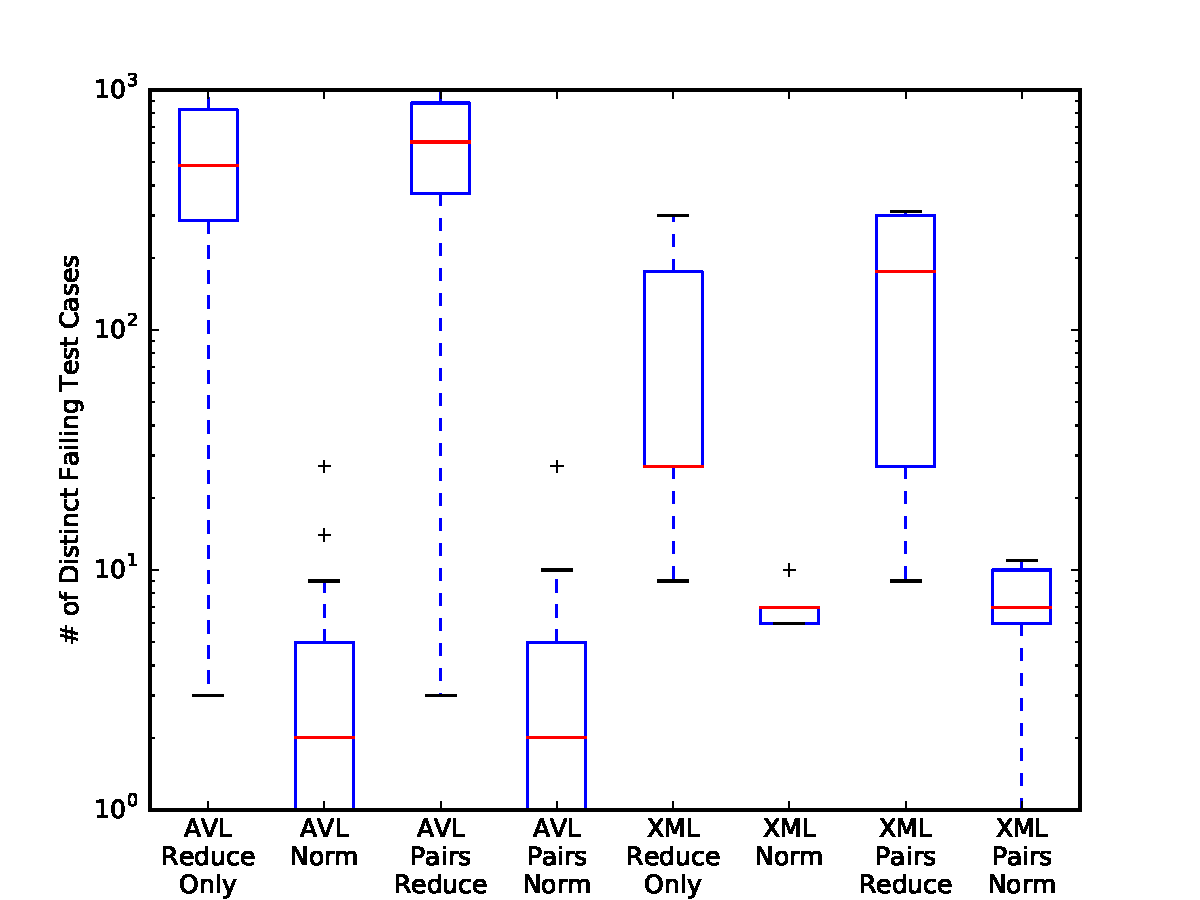
\includegraphics[width=\columnwidth]{length}
\caption{Effects of normalization on AVLTree and XML parser mutants.}
\label{normeffect}
\end{figure}

Figure \ref{normeffect} shows the reduction in number of distinct
failing tests produced by normalization and reduction
(vs. reduction only) for a set of 82 mutants \cite{mutant} of AVLTree
\cite{Hunter:2007} ({\bf RQ1}).  Of the 228 mutants produced by MutPy
\cite{mutpy}, only these 82 produced at least 1 failure in 1,000 tests (other mutants were equivalent or caused failure at a lower
rate).  Using reduction only, the mean number of distinct failures for
each mutant (obviously a single fault) was 498.4 (median 485).  Using normalization, the mean
was 3.1 failures (median 2).  For 38 of the 82 mutants,
normalization produced only a single failure.
Differences were statistically significant by paired Wilcoxon test with
$p\leq1\times10^{-15}$\footnote{All $p$-values given below are for
  the same recommended \cite{arcuri2014hitchhiker} statistical test.}.


AVLTree mutants also provided a way to evaluate the danger of
normalization losing faults, {\bf RQ2}.  Faults can be lost when normalization
changes a test failing due to one fault into a test failing
due to a different fault, a problem known as ``slippage''
\cite{PLDI13,slippage}.  AVLTree provides a slippage challenge, as there are
very few API calls, and all calls take the same inputs, so tests
for faults are likely to be very close to each other in the
combinatorial space.  To test the slippage rates for normalization, we
randomly selected 364 mutant pairs drawn from the 82 detectable
mutants, and produced higher-order-mutants for each of these by
applying both mutants to the source (using only mutants that modified
different source lines).  Of these, the set of reduced tests
included at least one test capable of exposing each of the two faults
for only 238 pairs.  In almost all cases this was due to reduction
slippage, but in a few cases it was due to one fault completely
masking another: e.g., if {\tt insert} always fails, it is not
possible to produce a test that exposes a fault in {\tt delete}
on a non-empty tree.

Out of these 238 mutant pairs, normalization produced tests
exposing both faults for 80.7\% of pairs (19.3\% slippage at the
suite level).  Interestingly, in 4 cases
normalization took a set of reduced tests not capable of exposing
both faults, and produced a smaller set of tests that was capable
of detecting both faults.  Slippage due to
reduction is very rare for some SUTs but common
for other SUTs (up to 23\% for Mozilla's JavaScript engine) \cite{PLDI13}.  For the AVLTree example, the slippage rate for reduction is almost 30\%,
10\% \emph{worse} than that for normalization.  Mitigation approaches
for slippage during reduction \cite{slippage} should also apply to normalization.

\begin{comment} Arguably this is ``slippage'' in that a test not
capable of exposing fault $F$ was modified to expose fault $F$ (classic
slippage) but since the new test suite exposed both faults,
normalization actually restored fault detection.

Data on slippage is not extensive, since it is only detected if the original test
cases before reduction are re-executed after bugs have been
fixed.  In our previous work \cite{PLDI13}, slippage due to
reduction was very rare for some SUTs (GCC 4.3.0) but common
for other SUTs (up to 23\% for Mozilla's JavaScript engine).  For the AVLTree example, the slippage rate for reduction is almost 30\%,
10\% \emph{worse} than that for normalization.  As a mitigation, we propose
storing reduced tests (and/or unreduced test
cases) as a slippage check when all faults detected by normalized test
cases are fixed.
\end{comment}

The reduction in tests produced by normalization for mutant pairs
was, as with single mutants, very large (Figure \ref{normeffect}).
For mutant pairs, the mean/median number of distinct failures was
554.4/607 for reduction alone, but only 2.8/2 with
normalization.  The runtime for normalization was almost
unchanged from the single-mutant times.  For reduction
alone, using pairs increased the number of distinct failures, while
normalized failure counts decreased.  For 48.3\% (115 of 238) of
mutant pairs where reduction did not lose a fault, normalization
worked as well as possible --- it preserved both faults and produced only 1 or 2 test
cases\footnote{It is sometimes possible to detect both faults with a single test
  case.}.  The improvement due to normalization was
statistically significant with $p\leq1\times10^{-80}$.
A second way to examine reduction in a multi-fault setting is to
consider the mean number of tests a user must examine before seeing
all faults \cite{PLDI13}.  For the AVL mutant pairs, a user must
examine almost 20 tests (on average) before encountering at least
one instance of both faults.  With normalization, this  drops
to a mean of just 2 tests.  The difference is significant with $p\leq1.4\times10^{-6}$.

AVLTree also provided basic results for {\bf RQ3}. The mean cost to reduce a
test was 0.05 seconds, with a median of 0.03 seconds.  The mean
cost for normalization was 0.38 seconds, with a median of 0.1 seconds.
The minimum runtime for both algorithms was negligible (less than 1
millisecond), but the maximums were 1.3 seconds for reduction and 17.6
seconds for normalization.  Note that in all our results the cost of
normalization is given on an already-reduced test, so the inputs
for normalization are smaller than those for reduction; however, this
is the expected use-case for normalization.  Comparing on equal-sized
tests would simply involve adding the costs for reduction to those for
normalization, as an additional step of normalization.  Finally, the
criticality of caching for normalizing large numbers of tests is
evident.  Out of 60,226 normalizations performed in our full AVLTree mutant
experiments, 59,972 (99.6\%) resulted in a cache hit (most of these
after a small number of normalization steps).  In fact, the total
number of rewrites performed during the experiments was only 145,780,
for a mean of only 2.4 non-cache-hit rewrites of each test.

\subsection{XML Parser}

We also investigated {\bf RQ1-3} for a
Python XML parser with about 260 lines of code \cite{myxml}, using one
real fault, triggered by the empty tag ({\tt <>}), and one
seeded fault triggered when adding two nodes with the same
name.  A comment in the code indicates the seeded fault is realistic,
and possibly existed in an earlier version of the code.  Running 1,000 tests
produced 848 failing tests.  Without normalization, it took only
37.45 seconds to execute and delta-debug all 1,000 tests.  The output was 717 distinct failing test
cases.  Normalization increased the runtime to 354.7 seconds, but
output only 5 failures (3 for the original fault and 2 for the seeded
fault).  The XML parser also shows that normalization and generalization work for
programs with string inputs defined by a grammar in TSTL, as well
as for
pure-API testing.
%reduced the number of failures to just 5: 3 
%for the original fault and 2 for the seeded fault.
%Generalization took < 5 seconds.

In addition to these realistic faults, we performed the same
mutation-based analysis as with AVLTree (Figure \ref{normeffect}). In
this case, a weaker specification (no reference implementation)
resulted in fault detection for only 5 of 357 mutants.  For these
mutants, reduction alone produced a mean of 107.6 failures (median
27); normalization reduced that to only 6.2 failures (median 7) ({\bf
  RQ1}).  The difference was significant at the 95\% confidence level,
($p=0.042$).  With mutant pairs, these numbers
increased to 181.9 mean faults (median 175) with reduction only,
compared to 7.7 mean faults (median 7) when using normalization ({\bf
  RQ1}).  This difference was statistically significant, 
$p=0.007$.  Normalization was perfect in only one case for
the XML parser mutants, and perfect for no mutant pairs.  The
difference in number of tests before encountering both faults
was not statistically significant (for these 5 faults,
failure rates are very similar, so hitting both is trivial).  For combined
mutants, the slippage rate was only 12.5\% for the XML parser ({\bf
  RQ2}).  That is, of the 9 viable mutant pairs, only 1 lost a fault,
and in that case the faults were both semantically and syntactically
very similar (within 1 line and with similar effects).  Reduction alone caused no slippage.  Adding normalization to reduction increased the runtime from
a mean of 12.6 seconds to 120.8 seconds ({\bf RQ3}); there were 3,829 cache hits over
a total of 3,929 normalizations.

\subsection{TSTL}

As noted in Section \ref{freshgen}, TSTL is used to test TSTL's own
API interface (the code is about 2,700 LOC; a compiled SUT is
often $>$ 30KLOC).  We discovered one fault while testing
the latest version of TSTL, the cache-related problem shown in Figure
\ref{fig:mislead}\footnote{We note that normalizing a test with
  respect to the predicate that it does not normalize (by a different
  predicate) may produce a headache in the TSTL user.}.
Generating and reducing 100 tests for it required 1,090 seconds
and produced 90 failures.  Normalization and generalization
increased total runtime to 3,690 seconds, and produced just 2
failures.

\subsection{SymPy}

\begin{figure}
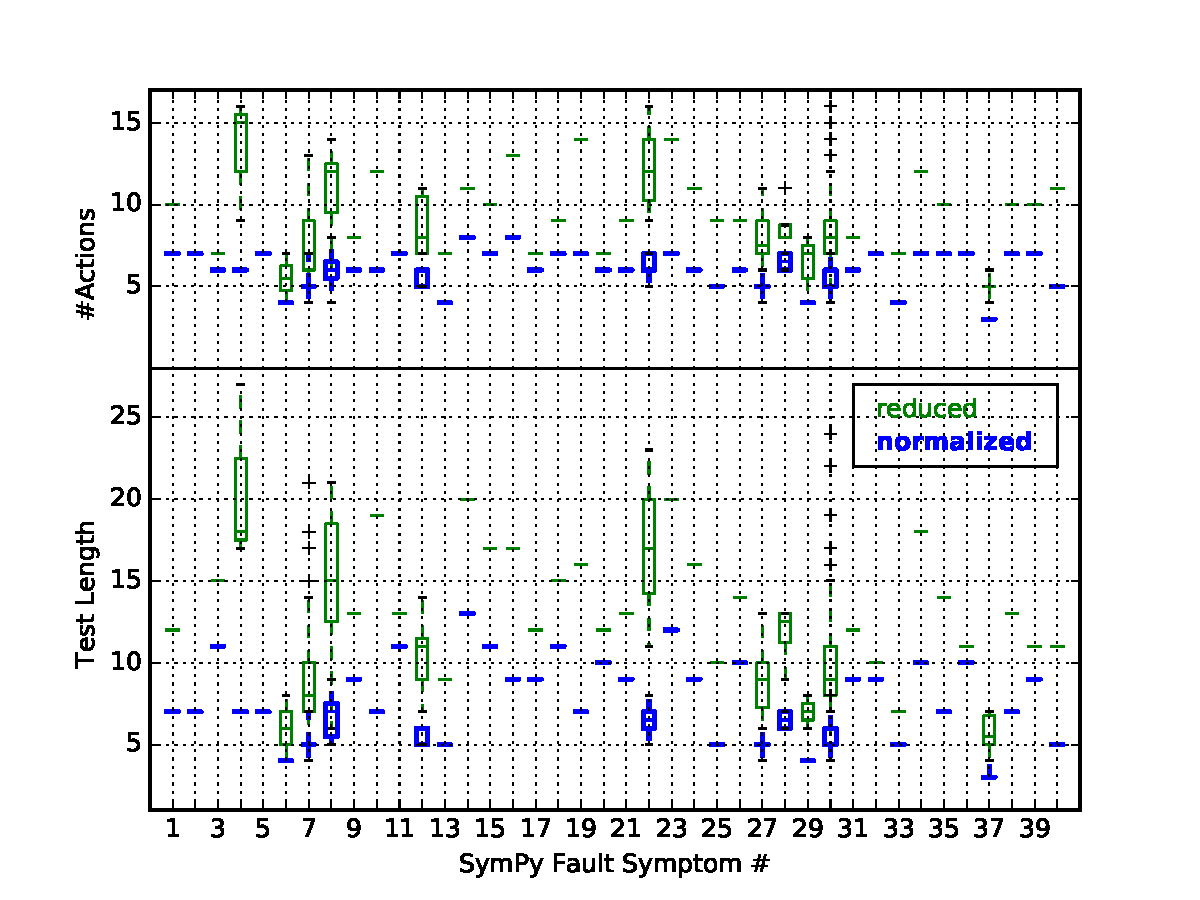
\includegraphics[width=\columnwidth]{sympyd}
\caption{Effects of normalization on SymPy tests.}
\label{lengthandactions}
\end{figure}

SymPy \cite{SymPy} is a widely used open source pure Python library
for symbolic mathematics.  SymPy is used by several other projects,
has over 400 contributors, over 25,000 commits to date, and over
225KLOC.  The TSTL tester for SymPy focuses on core expressions and
algebraic simplification, and covers about 15KLOC and 21,000 branches of
the system.  Testing this core resulted in discovery of a number
of faults in SymPy, detected by assertion violations or uncaught (and
not expected) exceptions.  Some of these have been reported to the project;
however, since SymPy currently has 2,128 open issues, with one opened
approximately each day, only one has (at this point) been fixed.  If we assume that
each different assertion violation or exception message indicates a
different underlying fault, SymPy provides us with a set of 40
complex, hard-to-understand real faults for evaluating normalization.
While we expect that this is an over-approximation of the actual
number of distinct faults, inspection of the tests and the covered
code suggests it is not far from the actual number.  Because we used a
(we believe)
non-lossy fault identification method (the exact failure symptom), our
SymPy results are relatively useless for {\bf RQ2}, but they answer {\bf RQ1}, {\bf RQ3}, and {\bf RQ4} for a large, realistic
system and real faults.

We generated, normalized, and reduced tests until we had 500 tests,
exhibiting all 40 fault signatures.    Some SymPy faults (not
included in our count of 40 tests) cause infinite loops, stopping
reduction or normalization. Of 570 failures, 549 reduced
and 500 both reduced and normalized.

{\bf RQ1:} Reduction alone did not reduce the number of distinct failing tests at
all.  Normalization reduced the total number of distinct
failing tests to 114.  There were
12.5 mean different failing tests, per fault, for both unreduced and
reduced tests, and only 3.15 mean failing tests per fault for
normalized tests.  This difference was significant, with $p=0.003$.
Normalization reduced the number of tests to
examine for 11 of the 13 faults with more than one failure; in 2 cases, the normalization was perfect (one failure).

{\bf RQ3:} The mean time for reduction was 104.45 seconds, with a
median of 19.70 seconds.  The mean time for normalization was
594 additional seconds, with a median of 260.214 seconds.  The
difference was significant, with $p\leq1\times10^{-80}$.

{\bf RQ4:} The mean length of unreduced tests was 44.664 steps, with a median
of 40.5 steps.  For reduced tests, this shrank to a mean of
9.984 and a median of 9.0 steps.  Normalized tests had mean length of
5.48 steps and median of 5.0 steps.  SymPy failures show
that normalization reduces not only the length of tests, but the number of
actions (roughly speaking, different API/method calls/functions) that must be considered for debugging:  reduced tests included
8.116 mean different actions, but normalized tests only 5.282
mean different actions.  These differences were all statistically
significant with $p\leq1\times10^{-76}$.  
Normalization made it possible to completely ignore a large number of
SymPy functions for debugging purposes.  The unreduced and reduced
tests included all 50 SymPy functions tested.  The normalized tests,
however, included only 32 of these, and enabled us to ignore such
complex code as trigonometric expansion and simplification, power expansion,
logarithmic combination, and even generalized expansion.  Figure
\ref{lengthandactions} graphically shows the impact of normalization
on length and number of functions covered by reduced tests.  The lower
part of the figure shows changes in test length, and the upper part
shows, for the same fault, the change in number of different actions.
The green boxplots show reduced tests, while the emphasized blue
boxplots show normalized tests.  It is clear that normalization not
only has a significant effect on average, but has a large benefit for
most individual faults.  The reduction in tests to examine
is also shown, indirectly, by the fact that the ``boxes'' for
normalized data are often simply lines because the tests are similar or identical.

\subsection{SortedContainers}

SortedContainers \cite{SortedContainers} is a popular Python library
of about 2KLOC, that provides pure Python sorted containers that are as fast as C
extension containers.  We have reported 3 bugs in SortedContainers
(all quickly corrected).  One of these bugs causes an infinite loop,
making it difficult to reduce or normalize.  We therefore only present
results for the other two faults reported.  We
generated 168 failing tests, all distinct, exhibiting both reported
faults, over 15 hours of testing. All failures reduced and normalized.
{\bf RQ1-RQ3:} Reduction did not reduce
the number of failures, but did reduce mean test length from
80.8 to 13.2 steps (median from 85.0 to 12.5), and mean number of
different actions per test from 14.4 to 7.4 (median from 14.0 to 8.0).
Normalization was perfect:  all tests normalized to two canonical
tests, one per fault, both with only 6 steps and 5
distinct actions --- a $>$ 50\% reduction in size beyond delta-debugging.  Changes were significant with
$p\leq1.0\times10^{-24}$.  There were 95 total
different actions in tests before reduction, 27 in tests after
reduction, and only 7 between the two normalized tests.  {\bf RQ4:} Reduction took a mean of 0.09 seconds, normalization a mean of 134.1
seconds (median 0.06 vs. 57.0) (significant, $p\leq1\times10^{-28}$).  

\subsection{NumPy}

\begin{comment}
\begin{figure}[t]
{\scriptsize
\begin{code}
 dim1 = 1                                       \# STEP 0
 shape2 = (dim1, dim1, dim1)                    \# STEP 1
 array1 = np.ones(shape2)                       \# STEP 2
 array0 = array1 * array1                       \# STEP 3
 array1 = array1 + array1                       \# STEP 4
 array4 = array0 + array1                       \# STEP 5
 array0 = np.reshape(array4,shape2)             \# STEP 6 
 array3 = array1 * array4                       \# STEP 7
 array2 = np.ravel(array4)                      \# STEP 8
 array5 = array2 - array3                       \# STEP 9 
 array4 = array5 * array2                       \# STEP 10
 array1 = np.unique(array0)                     \# STEP 11
 array5 = array5 * array3                       \# STEP 12
 array0 = array1 * array5                       \# STEP 13
 array5 = np.unique(array0)                     \# STEP 14
 array1 = array4 - array2                       \# STEP 15
 array2 = array0.flatten()                      \# STEP 16
 array0 = array5 + array5                       \# STEP 17
 array5 = array5 + array2                       \# STEP 18
 array2 = array0 * array2                       \# STEP 19
 np.copyto(array5,array2)                       \# STEP 20
 array2 = array2 * array5                       \# STEP 21
 array3 = array0 * array2                       \# STEP 22
 array0 = array3 - array1                       \# STEP 23
 array4 = array3 * array0                       \# STEP 24
 array1 = array5 + array4                       \# STEP 25
 array5 = array0 * array1                       \# STEP 26
 array0 = array5 - array1                       \# STEP 27
 array4 = array0 * array3                       \# STEP 28
 array3 = array4 * array0                       \# STEP 29
 array1 = array5 + array3                       \# STEP 30
 array0 = array2 + array1                       \# STEP 31
 array5 = array5 - array0                       \# STEP 32
 array5 = array3 * array5                       \# STEP 33
 array0 = array1 + array5                       \# STEP 34
 array2 = array3 - array0                       \# STEP 35
 array4 = array2 * array1                       \# STEP 36
 array3 = array4 * array2                       \# STEP 37
 array2 = array0 - array0                       \# STEP 38
 np.copyto(array1,array3)                       \# STEP 39
 array4 = array2.flatten()                      \# STEP 40
 array1 = array1 * array4                       \# STEP 41
 assert (np.array\_equal(array1,array1))
\end{code}
}
\caption{Reduced () ``failing'' test for NumPy.}
\label{numpyorig}
\end{figure}
\end{comment}

Our final two case studies provide little information on {\bf RQ1} and
{\bf RQ2}; for these SUTs, failure rates are low enough or test
reduction runtimes high enough that each failure is usually dealt with
one-by-one.  However, the value of normalization and generalization
for further reduction ({\bf RQ4}) and aiding in understanding tests ({\bf
  RQ5}) is effectively shown by these complex programs.  They also provide
results for {\bf RQ3} when even test reduction is expensive.
NumPy \cite{NumPy} is a widely used Python library that
supports large, multi-dimensional matrices and provides a huge library
of mathematical functions.  The SciPy library for scientific
computing builds on NumPy.  Developing tests for NumPy is challenging,
because none of the authors are experts in numeric computation, and
the specification of correct behavior is often somewhat subtle.  As an
example, consider the test in Figure \ref{numpynormgen}.  Prior to
normalization, understanding why the test leads to a violation of
self-equality for an array is difficult: the reduced-only test has 42
steps and includes not only array multiplication and addition, but
subtraction, array copying, reshaping, flattening,  filtering by
unique elements, and raveling.  After
normalization, it is much clearer what is happening: 1) {\tt array0}
contains {\tt NaN} and 2) this is correct behavior (the array
\emph{should} contain {\tt NaN}).  The greater length and much larger
number of operations involved in the original reduced test
obscures this critical point.  In NumPy, array equality does not hold
for objects containing {\tt NaN}, so the assertion must be modified.
As far as we know, normalization transforms all instances of this
fault into this canonical test, but our data is insufficient to make a definite claim.

Other, more complex, failures have also made it clear that
normalization is useful for additional test length reduction for
NumPy, and that generalization makes any surprising restrictions on
test values clear.  For NumPy tests, normalization takes much longer
than reduction, in part due to the expense of operations on large
arrays.  For almost all tests, the mean time to reduce tests
is about 4-5 seconds, and the time for normalization is between 712
and 774 seconds.   Generalization takes
between 52 and 59 seconds in these cases.  The exception was a test of 45,206 steps (!)  leading to a memory exhaustion error and
crash.  This was reduced (over nearly a day) to a test
with 10 steps, which then normalized (in only 2 hours) to a test
with 8 steps.  The normalized test involved no operations other than array
initialization, array flattening, and array
addition.  The reduced test involved larger array dimensions, array
multiplication, and array subtraction, as well.  
%This is the only case in
%which we have seen normalization time lower than reduction time,
%without assistance from the cache.



\begin{figure}
{\scriptsize
\begin{code}
dim0 = 1                            \textcolor{black!60}{\# STEP 0}
\textcolor{black!60}{\#  or dim0 = 10 }
shape0 = (dim0)                     \textcolor{black!60}{\# STEP 1}
\textcolor{black!60}{\#  or shape0 = (dim0, dim0) }
\textcolor{black!60}{\#  or shape0 = (dim0, dim0, dim0) }
array0 = np.ones(shape0)            \textcolor{black!60}{\# STEP 2}
array0 = array0 + array0            \textcolor{black!60}{\# STEP 3}
array0 = array0 + array0            \textcolor{black!60}{\# STEP 4}
\textcolor{black!60}{\#  or array0 = array0 * array0 }
array0 = array0 * array0            \textcolor{black!60}{\# STEP 5}
array0 = array0 * array0            \textcolor{black!60}{\# STEP 6}
array0 = array0 * array0            \textcolor{black!60}{\# STEP 7}
array0 = array0 * array0            \textcolor{black!60}{\# STEP 8}
array0 = array0 * array0            \textcolor{black!60}{\# STEP 9}
array0 = array0 * array0            \textcolor{black!60}{\# STEP 10}
array0 = array0 * array0            \textcolor{black!60}{\# STEP 11}
array0 = array0 * array0            \textcolor{black!60}{\# STEP 12}
array0 = array0 * array0            \textcolor{black!60}{\# STEP 13}
array0 = array0 - array0            \textcolor{black!60}{\# STEP 14}
assert (np.array\_equal(array0,array0))
\end{code}
}
\caption{Normalized and generalized NumPy test.}
\label{numpynormgen}
\end{figure}

\subsection{Esri ArcPy}

Esri is the single
largest Geographic Information System (GIS) software vendor.  Esri's ArcGIS tools are widely
used for GIS analysis.  Automation is essential for complex GIS analysis and
data management, and Esri has long provided tools
for programming GIS software systems.  One such tool
is a Python site-package, ArcPy \cite{ArcPy}.  ArcPy is a complex library,
with dozens of classes and hundreds of functions.  Most of the code involved in ArcPy
functionality is the C++ source for ArcGIS itself (which is not
available), but the released Python interface code alone is over 50KLOC.
We have  discovered and reported six crash-inducing faults in
ArcPy/ArcGIS.  
%It is critical to understand these
%faults and the behaviors that trigger them to modify the harness to
%avoid triggering these faults, while restricting other testing as
%little as possible.

%There is no space in this paper to elaborate on the details of this
%large test effort (which has introduced numerous additional features
%and modes to TSTL), but normalization and generalization have been
%very useful in this process.  

Figures \ref{esriorig} and
\ref{esrinormgen} show one crash-inducing test, after initial
delta-debugging (from over 2,000 test steps) (Figure \ref{esriorig})
and after normalization and generalization (Figure \ref{esrinormgen}).
In this setting normalization has contributed a significant amount of
additional reduction over delta-debugging.  For the crash fault shown
in this paper, normalization reduced the length from 19 steps to 11
steps.  For three other crashes, normalization reduced the tests
from 18 to 14 steps, from 27 to 20 steps, and from 20 to 16 steps. One crash fault only reduced from 10 steps to 9 steps, but the
omission was informative.  None of the ArcPy faults experienced slippage --- the normalized
test was always clearly the same fault as the reduced test.
 The cost of normalization is high --- in
our runs, it has taken from 17,340 seconds up to 24,769 seconds.
However, in this setting even delta-debugging is extremely expensive
--- the cost of reduction alone has ranged from 7,930 seconds to 8,688
seconds.  Generalization has taken between 3,203 and
 11,149 seconds.  These high costs are due to the need to run
tests in a sandbox environment to avoid killing the testing
process, and the runtime of complex GIS analyses.
Even under these circumstances, reducing, normalizing, and
generalizing tests has been a more effective use of human time than
trying to understand the faults without help.  For example, in
the test shown in this paper, it was important to understand that
the SQL query and selection type are not essential, but using a
freshly created layer will not result in a crash: the problem appears
to be that ArcGIS (or ArcPy) does not invalidate layers built from a
feature class when that feature class is deleted.  In this
  instance, a generalization (the fresh values generalization in
  particular) is informative by its absence: we know that it was attempted, but prevented
  failure.  The reduced, non-normalized test (Figure \ref{esriorig})
makes this far less clear, as the use of {\tt CopyFeatures} and the
multiplicity of shapefiles involved disguises the essence of the
problem.  

We are also preparing a test suite that covers as much as
possible of the Python source in the latest version of ArcPy
and records the values returned.  For future versions of ArcPy, a ``semantic diff'' based on these calls
can be produced, allowing developers to see how API usage changes with
new releases.  The tests in the suite are
normalized and generalized (based on code coverage and output, not
failure --- these tests all pass) to make them easy to understand, and show
which parameter combinations do not change results.


\begin{comment}
Normalization and generalization are also being used to prepare an
API-behavior regression suite for ArcPy.  One of the challenges of
using a large API like ArcPy is that behavior of the system can change
from version to version.  In some cases this is due to new faults, or
fixed faults, but in other cases there is an undocumented usage change.  To assist ArcPy
developers, we are preparing a test suite that covers as much as
possible of the Python source in the latest version of ArcPy
and records the values returned.  For future versions of ArcPy, a ``semantic diff'' based on these calls
can be produced.  The tests in the suite are
normalized and generalized to help users understand API usage
consequences, since Esri examples are limited to simple parameter
combinations, and many illegal combinations are not specified.
\end{comment}

\begin{figure}[t]
{\scriptsize 
\begin{code}
shapefile2 = "C:\\arctmp\\new3.shp"                \# STEP 0 
shapefile1 = "C:\\arctmp\\new3.shp"                \# STEP 1
featureclass2 = shapefile2                       \# STEP 2
featureclass0 = shapefile1                       \# STEP 3
shapefilelist2 = 
   glob.glob("C:\\Arctmp\\*.shp")                  \# STEP 4
fieldname0 = "newf3"                             \# STEP 5
shapefile1 = shapefilelist2 [0]                  \# STEP 6
featureclass1 = shapefile1                       \# STEP 7
arcpy.CopyFeatures\_management
   (featureclass1,featureclass2)                 \# STEP 8
op1 = ">"                                        \# STEP 9
newlayer2 = "l2"                                 \# STEP 10
val1 = "100"                                     \# STEP 11
selectiontype2 = "SWITCH\_SELECTION"              \# STEP 12
fieldname1 = "newf1"                             \# STEP 13
arcpy.MakeFeatureLayer\_management
   (featureclass0, newlayer2)                    \# STEP 14
arcpy.SelectLayerByAttribute\_management
   (newlayer2,selectiontype2,
   ' "'+fieldname0+'" '+op1+val1)                \# STEP 15
op0 = ">"                                        \# STEP 16
arcpy.Delete\_management(featureclass2)           \# STEP 17
arcpy.SelectLayerByAttribute\_management
   (newlayer2,selectiontype2,
   ' "'+fieldname1+'" '+op0+val1)                \# STEP 18
\end{code}
}
\caption{Test with reduction-only for ArcPy.}
%\vspace{-0.33in}
\label{esriorig}
\end{figure}

\begin{figure}[t]
{\scriptsize 
\begin{code}
shapefilelist0 = 
   glob.glob("C:\\Arctmp\\*.shp")        \textcolor{black!60}{\# STEP 0}
\textcolor{black!60}{\#[}
shapefile0 = shapefilelist0 [0]        \textcolor{black!60}{\# STEP 1}
newlayer0 = "l1"                       \textcolor{black!60}{\# STEP 2}
\textcolor{black!60}{\#  or newlayer0 = "l2" }
\textcolor{black!60}{\#  or newlayer0 = "l3" }
\textcolor{black!60}{\#  swaps with steps 3 4 5 6 7}
\textcolor{black!60}{\#] (steps in [] can be in any order)}
\textcolor{black!60}{\#[}
featureclass0 = shapefile0             \textcolor{black!60}{\# STEP 3}
\textcolor{black!60}{\#  swaps with step 2}
fieldname0 = "newf1"                   \textcolor{black!60}{\# STEP 4}
\textcolor{black!60}{\#  or fieldname0 = "newf2" }
\textcolor{black!60}{\#  or fieldname0 = "newf3" }
\textcolor{black!60}{\#  swaps with steps 2 8}
selectiontype0 = "SWITCH\_SELECTION"    \textcolor{black!60}{\# STEP 5}
\textcolor{black!60}{\#  or selectiontype0 = "NEW\_SELECTION" }
\textcolor{black!60}{\#  or selectiontype0 = "ADD\_TO\_SELECTION" }
\textcolor{black!60}{\#  or selectiontype0 = "REMOVE\_FROM\_SELECTION"}
\textcolor{black!60}{\#  or selectiontype0 = "SUBSET\_SELECTION"}
\textcolor{black!60}{\#  or selectiontype0 = "CLEAR\_SELECTION"   }
\textcolor{black!60}{\#  swaps with steps 2 8}
op0 = ">"                              \textcolor{black!60}{\# STEP 6}
\textcolor{black!60}{\#  or op0 = "<" }
\textcolor{black!60}{\#  swaps with steps 2 8}
val0 = "100"                           \textcolor{black!60}{\# STEP 7}
\textcolor{black!60}{\#  or val0 = "1000" }
\textcolor{black!60}{\#  swaps with steps 2 8}
\textcolor{black!60}{\#] (steps in [] can be in any order)}
arcpy.MakeFeatureLayer\_management
   (featureclass0, newlayer0)          \textcolor{black!60}{\# STEP 8}
\textcolor{black!60}{\#  swaps with steps 4 5 6 7}
arcpy.SelectLayerByAttribute\_management
   (newlayer0,selectiontype0,
   ' "'+fieldname0+'" '+op0+val0)      \textcolor{black!60}{\# STEP 9}
arcpy.Delete\_management(featureclass0) \textcolor{black!60}{\# STEP 10}
arcpy.SelectLayerByAttribute\_management
   (newlayer0,selectiontype0,
   ' "'+ fieldname0+'" '+op0+val0)     \textcolor{black!60}{\# STEP 11}
\end{code}
}
\caption{Normalized and generalized ArcPy test.}
\label{esrinormgen}
\end{figure}
